% Options for packages loaded elsewhere
\PassOptionsToPackage{unicode}{hyperref}
\PassOptionsToPackage{hyphens}{url}
%
\documentclass[
  17pt,
  letterpaper,
  ignorenonframetext,
  aspectratio=169,
  handout,
  xcolor={dvipsnames}]{beamer}
\usepackage{pgfpages}
\setbeamertemplate{caption}[numbered]
\setbeamertemplate{caption label separator}{: }
\setbeamercolor{caption name}{fg=normal text.fg}
\beamertemplatenavigationsymbolsempty
% Prevent slide breaks in the middle of a paragraph
\widowpenalties 1 10000
\raggedbottom
\setbeamertemplate{part page}{
  \centering
  \begin{beamercolorbox}[sep=16pt,center]{part title}
    \usebeamerfont{part title}\insertpart\par
  \end{beamercolorbox}
}
\setbeamertemplate{section page}{
  \centering
  \begin{beamercolorbox}[sep=12pt,center]{part title}
    \usebeamerfont{section title}\insertsection\par
  \end{beamercolorbox}
}
\setbeamertemplate{subsection page}{
  \centering
  \begin{beamercolorbox}[sep=8pt,center]{part title}
    \usebeamerfont{subsection title}\insertsubsection\par
  \end{beamercolorbox}
}
\AtBeginPart{
  \frame{\partpage}
}
\AtBeginSection{
  \ifbibliography
  \else
    \frame{\sectionpage}
  \fi
}
\AtBeginSubsection{
  \frame{\subsectionpage}
}

\usepackage{amsmath,amssymb}
\usepackage{lmodern}
\usepackage{iftex}
\ifPDFTeX
  \usepackage[T1]{fontenc}
  \usepackage[utf8]{inputenc}
  \usepackage{textcomp} % provide euro and other symbols
\else % if luatex or xetex
  \usepackage{unicode-math}
  \defaultfontfeatures{Scale=MatchLowercase}
  \defaultfontfeatures[\rmfamily]{Ligatures=TeX,Scale=1}
  \setmainfont[BoldFont = SF Pro Text Semibold, Scale =
MatchLowercase]{SF Pro Text Light}
\fi
\usecolortheme{wolverine}
\usefonttheme{serif} % use mainfont rather than sansfont for slide text
\useinnertheme{default}
\useoutertheme{miniframes}
% Use upquote if available, for straight quotes in verbatim environments
\IfFileExists{upquote.sty}{\usepackage{upquote}}{}
\IfFileExists{microtype.sty}{% use microtype if available
  \usepackage[]{microtype}
  \UseMicrotypeSet[protrusion]{basicmath} % disable protrusion for tt fonts
}{}
\makeatletter
\@ifundefined{KOMAClassName}{% if non-KOMA class
  \IfFileExists{parskip.sty}{%
    \usepackage{parskip}
  }{% else
    \setlength{\parindent}{0pt}
    \setlength{\parskip}{6pt plus 2pt minus 1pt}}
}{% if KOMA class
  \KOMAoptions{parskip=half}}
\makeatother
\usepackage{xcolor}
\newif\ifbibliography
\setlength{\emergencystretch}{3em} % prevent overfull lines
\setcounter{secnumdepth}{-\maxdimen} % remove section numbering


\providecommand{\tightlist}{%
  \setlength{\itemsep}{0pt}\setlength{\parskip}{0pt}}\usepackage{longtable,booktabs,array}
\usepackage{calc} % for calculating minipage widths
\usepackage{caption}
% Make caption package work with longtable
\makeatletter
\def\fnum@table{\tablename~\thetable}
\makeatother
\usepackage{graphicx}
\makeatletter
\def\maxwidth{\ifdim\Gin@nat@width>\linewidth\linewidth\else\Gin@nat@width\fi}
\def\maxheight{\ifdim\Gin@nat@height>\textheight\textheight\else\Gin@nat@height\fi}
\makeatother
% Scale images if necessary, so that they will not overflow the page
% margins by default, and it is still possible to overwrite the defaults
% using explicit options in \includegraphics[width, height, ...]{}
\setkeys{Gin}{width=\maxwidth,height=\maxheight,keepaspectratio}
% Set default figure placement to htbp
\makeatletter
\def\fps@figure{htbp}
\makeatother

\captionsetup[figure]{labelformat=empty}
\usepackage{pgfpages}
\setbeamertemplate{itemize item}[circle]
\setbeamertemplate{footline}[frame number]{}
\mode<handout>{\pgfpagesuselayout{6 on 1}[letterpaper, border shrink=8mm]}
\AtBeginSection{%
   \begin{frame}
       \tableofcontents[currentsection]
   \end{frame}
}
\makeatletter
\makeatother
\makeatletter
\makeatother
\makeatletter
\@ifpackageloaded{caption}{}{\usepackage{caption}}
\AtBeginDocument{%
\ifdefined\contentsname
  \renewcommand*\contentsname{Table of contents}
\else
  \newcommand\contentsname{Table of contents}
\fi
\ifdefined\listfigurename
  \renewcommand*\listfigurename{List of Figures}
\else
  \newcommand\listfigurename{List of Figures}
\fi
\ifdefined\listtablename
  \renewcommand*\listtablename{List of Tables}
\else
  \newcommand\listtablename{List of Tables}
\fi
\ifdefined\figurename
  \renewcommand*\figurename{Figure}
\else
  \newcommand\figurename{Figure}
\fi
\ifdefined\tablename
  \renewcommand*\tablename{Table}
\else
  \newcommand\tablename{Table}
\fi
}
\@ifpackageloaded{float}{}{\usepackage{float}}
\floatstyle{ruled}
\@ifundefined{c@chapter}{\newfloat{codelisting}{h}{lop}}{\newfloat{codelisting}{h}{lop}[chapter]}
\floatname{codelisting}{Listing}
\newcommand*\listoflistings{\listof{codelisting}{List of Listings}}
\makeatother
\makeatletter
\@ifpackageloaded{caption}{}{\usepackage{caption}}
\@ifpackageloaded{subcaption}{}{\usepackage{subcaption}}
\makeatother
\makeatletter
\@ifpackageloaded{tcolorbox}{}{\usepackage[many]{tcolorbox}}
\makeatother
\makeatletter
\@ifundefined{shadecolor}{\definecolor{shadecolor}{rgb}{.97, .97, .97}}
\makeatother
\makeatletter
\makeatother
\ifLuaTeX
  \usepackage{selnolig}  % disable illegal ligatures
\fi
\IfFileExists{bookmark.sty}{\usepackage{bookmark}}{\usepackage{hyperref}}
\IfFileExists{xurl.sty}{\usepackage{xurl}}{} % add URL line breaks if available
\urlstyle{same} % disable monospaced font for URLs
\hypersetup{
  pdftitle={Knowledge and Reality, Lecture 19},
  pdfauthor={Brian Weatherson},
  hidelinks,
  pdfcreator={LaTeX via pandoc}}

\title{Knowledge and Reality, Lecture 19}
\author{Brian Weatherson}
\date{11/7/22}

\begin{document}
\frame{\titlepage}
\ifdefined\Shaded\renewenvironment{Shaded}{\begin{tcolorbox}[boxrule=0pt, sharp corners, breakable, borderline west={3pt}{0pt}{shadecolor}, frame hidden, enhanced, interior hidden]}{\end{tcolorbox}}\fi

\hypertarget{experience}{%
\section{Experience}\label{experience}}

\begin{frame}{Big Question}
\protect\hypertarget{big-question}{}
Is experience sensitive to background beliefs, skills, or dispositions?
\end{frame}

\begin{frame}{Argument from Illusion}
\protect\hypertarget{argument-from-illusion}{}
Here is one reason to think that it is not.

\begin{itemize}[<+->]
\tightlist
\item
  We see illusions the way they are `meant' to be seen even when we know
  better.
\end{itemize}

\end{frame} \begin{frame}[plain]

\begin{figure}

{\centering 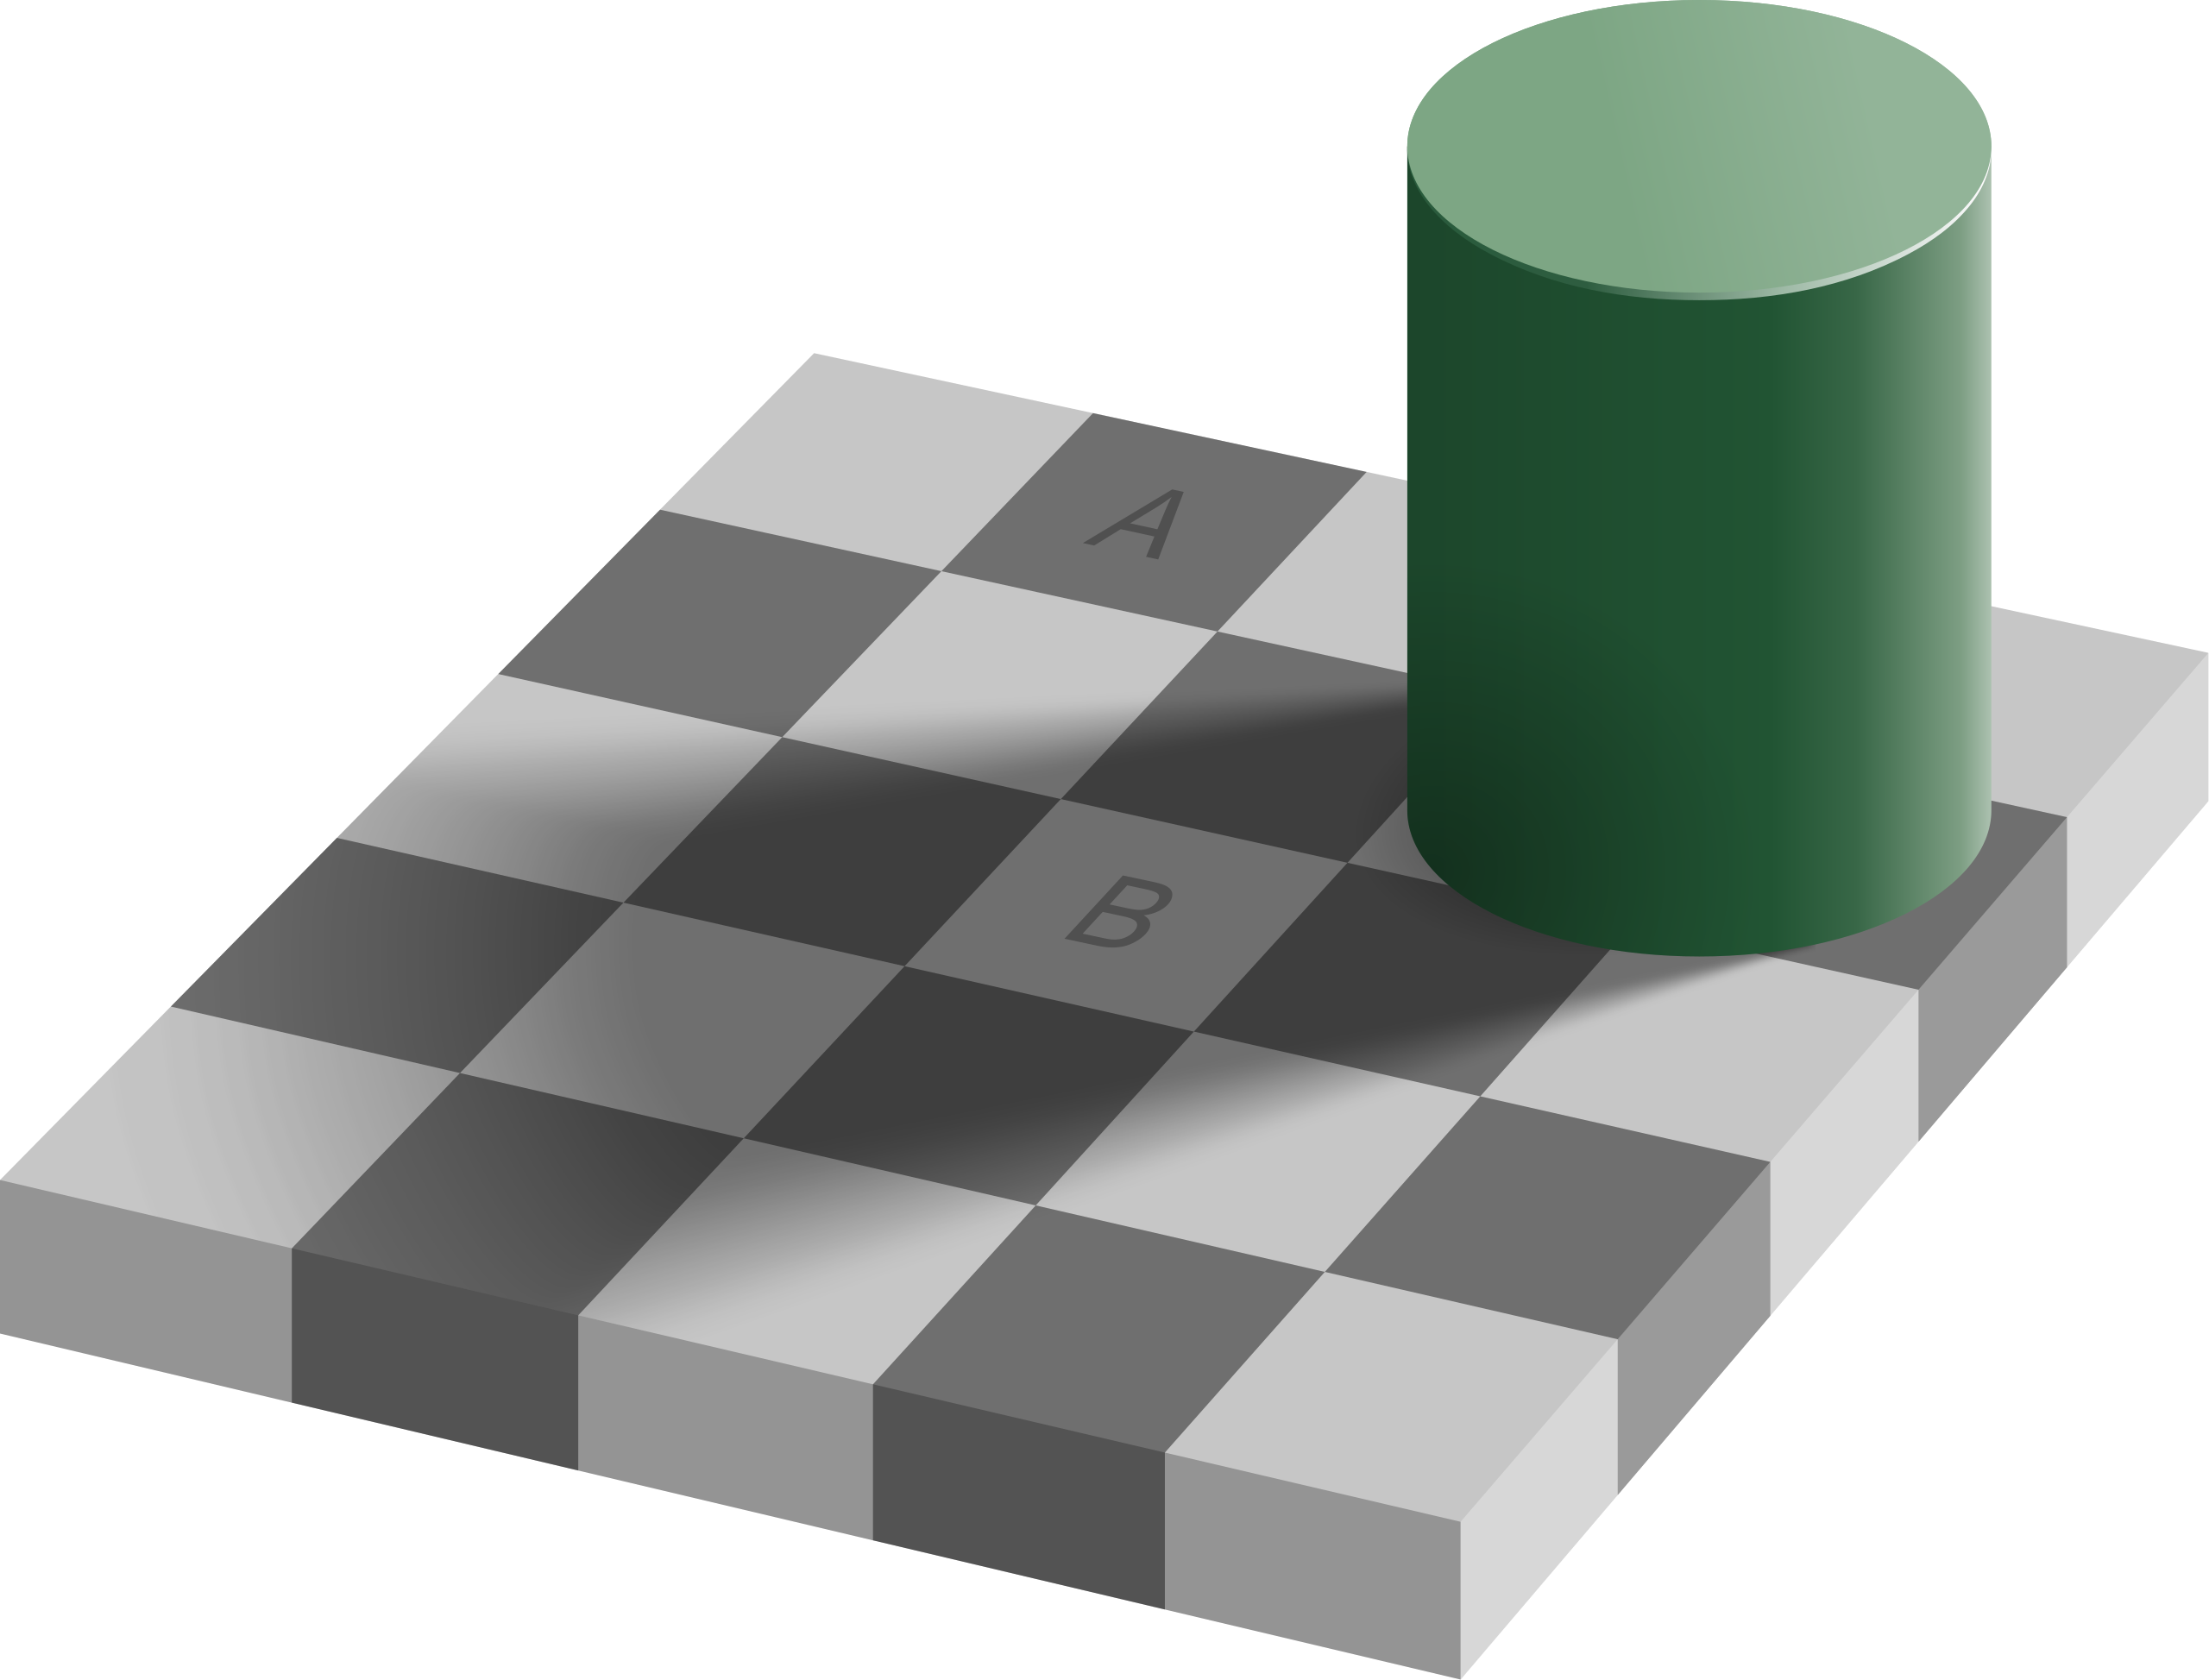
\includegraphics[width=\textwidth,height=0.8\textheight]{../images/checker_shadow.png}

}

\caption{Edward Adelson's checker-shadow illusion}

\end{figure}
\end{frame}

\begin{frame}{Checker Shadow}
\protect\hypertarget{checker-shadow}{}
\begin{enumerate}[<+->]
\tightlist
\item
  The squares A and B are the same shade on the page.
\item
  They don't look that way!
\item
  They stay not looking that way even when you know better.
\end{enumerate}

\end{frame} \begin{frame}[plain]

\begin{figure}

{\centering 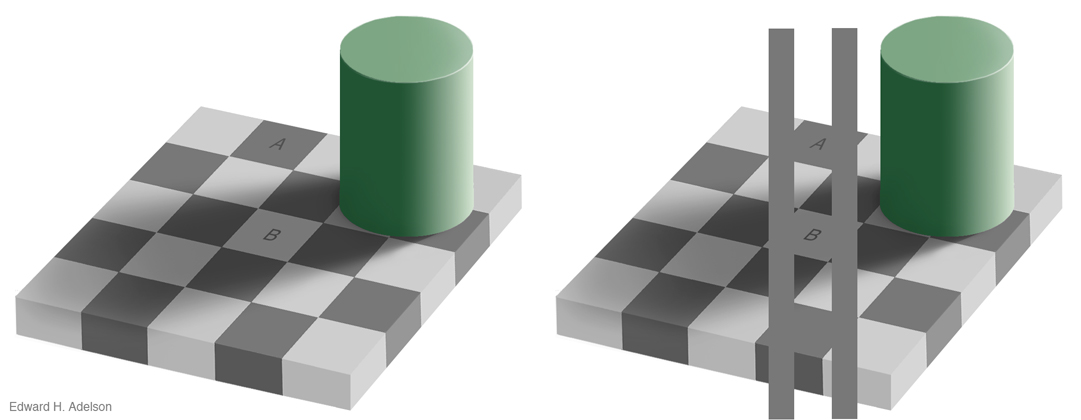
\includegraphics[width=\textwidth,height=0.8\textheight]{../images/checkershadow_double.jpg}

}

\caption{Showing that A and B are the same}

\end{figure}
\end{frame}

\begin{frame}{Argument}
\protect\hypertarget{argument}{}
\begin{enumerate}[<+->]
\tightlist
\item
  If experience were penetrated by belief, then once we believed A and B
  were the same, they'd look the same.
\item
  They don't look the same, even once we know they are.
\end{enumerate}

\begin{enumerate}[<+->]
[A.]
\setcounter{enumi}{2}
\tightlist
\item
  So, experience isn't penetrated by belief
\end{enumerate}
\end{frame}

\begin{frame}{What's Wrong with this Argument}
\protect\hypertarget{whats-wrong-with-this-argument}{}
It just shows that a certain kind of penetration doesn't work.

\begin{itemize}[<+->]
\tightlist
\item
  Lots of other ways for belief to affect experience other than that.
\end{itemize}
\end{frame}

\begin{frame}[plain]{Memorisation Test}
\protect\hypertarget{memorisation-test}{}
\begin{figure}

{\centering 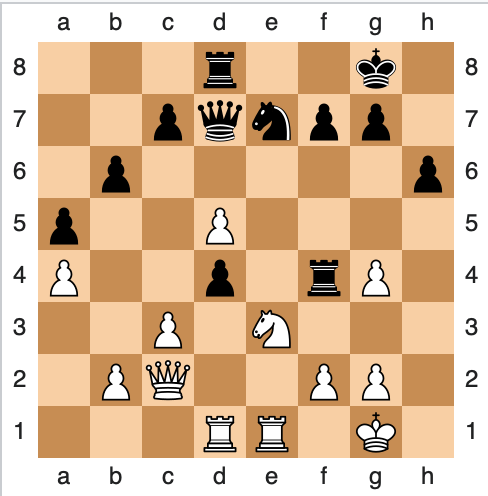
\includegraphics[width=\textwidth,height=0.8\textheight]{../images/chess_gm11.png}

}

\caption{The position after move 22 in game 11 of 2021 World
Championship}

\end{figure}
\end{frame}

\begin{frame}{Two Empirical Claims}
\protect\hypertarget{two-empirical-claims}{}
\begin{enumerate}[<+->]
\tightlist
\item
  Expert chess players do much better at remembering that position after
  seeing it for a few seconds than the rest of us. (Not including you if
  you're an expert!)
\item
  They aren't \emph{much} better at memorising boards where pieces are
  just randomly spread around a board.
\end{enumerate}
\end{frame}

\begin{frame}{Hypothesis}
\protect\hypertarget{hypothesis}{}
\begin{enumerate}[<+->]
\tightlist
\item
  Chess players see the board as a game state, and hence remember it
  better.
\item
  That doesn't work for random distributions, except to the extent that
  some of the pieces fall into game-like distributions.
\end{enumerate}
\end{frame}

\begin{frame}{Stroop Effect}
\protect\hypertarget{stroop-effect}{}
It's really hard - I mean \emph{really} hard - to perceive words in
languages you can read as anything other than words.

\begin{itemize}[<+->]
\tightlist
\item
  On the next slide, say (to yourself) as quickly as possible the colors
  that each word is written in.
\end{itemize}

\end{frame} \begin{frame}[plain]

\begin{columns}[T]
\begin{column}{0.25\textwidth}
\LARGE{ \textcolor{Blue}{Blue} \\ \textcolor{Brown}{Brown}  \\ \textcolor{ForestGreen}{Green} }
\end{column}

\begin{column}{0.25\textwidth}
\LARGE{  \textcolor{Purple}{Purple}    \\  \textcolor{BrickRed}{Red}    \\     \textcolor{Yellow}{Yellow} }
\end{column}

\begin{column}{0.25\textwidth}
\LARGE{  \textcolor{Aquamarine}{Teal} \\  \textcolor{Black}{Black} \\  \textcolor{Rhodamine}{Pink} }
\end{column}
\end{columns}

\end{frame} \begin{frame}[plain]

Let's try it again, with some rotations.

\end{frame} \begin{frame}[plain]

\begin{columns}[T]
\begin{column}{0.25\textwidth}
\LARGE{ \textcolor{Blue}{Red} \\ \textcolor{Brown}{Yellow}  \\ \textcolor{ForestGreen}{Teal} }
\end{column}

\begin{column}{0.25\textwidth}
\LARGE{  \textcolor{Purple}{Black}    \\  \textcolor{BrickRed}{Pink}    \\     \textcolor{Yellow}{Blue} }
\end{column}

\begin{column}{0.25\textwidth}
\LARGE{  \textcolor{Aquamarine}{Brown} \\  \textcolor{Black}{Green} \\  \textcolor{Rhodamine}{Purple} }
\end{column}
\end{columns}
\end{frame}

\begin{frame}{Hijacking}
\protect\hypertarget{hijacking}{}
Typically, people who can read English will do worse on this than people
who cannot.

\begin{itemize}[<+->]
\tightlist
\item
  If you can read English, your perception of the words will hijack your
  color perception.
\item
  Again, feels like something is getting in the way of perception.
\end{itemize}
\end{frame}

\begin{frame}{Big Picture}
\protect\hypertarget{big-picture}{}
\begin{itemize}[<+->]
\tightlist
\item
  Something in background effects how things look.
\item
  That effect is evaluable.
\item
  If it is both bad for accuracy and not supported by evidence, it seems
  to make the perception itself irrational.
\end{itemize}
\end{frame}

\hypertarget{inference-and-rationality}{%
\section{Inference and Rationality}\label{inference-and-rationality}}

\begin{frame}{Siegel's Picture}
\protect\hypertarget{siegels-picture}{}
\begin{enumerate}[<+->]
\tightlist
\item
  Experiences are the product of (something like) inference.
\item
  The products of inference are assessable as rational/irrational.
\end{enumerate}

\begin{enumerate}[<+->]
[A.]
\setcounter{enumi}{2}
\tightlist
\item
  Experiences are assessable as rational/irrational.
\end{enumerate}
\end{frame}

\begin{frame}{Evaluating Inferences}
\protect\hypertarget{evaluating-inferences}{}
\begin{itemize}[<+->]
\tightlist
\item
  In theory, can ask about whether the premises are well-supported, and
  about whether the inference follows from the premises.
\item
  In practice, hard to make this distinction out.
\item
  Everyone who looks like they are reasoning in a way that doesn't
  follow could be implicitly believing ``If premises, then conclusion.''
\end{itemize}
\end{frame}

\begin{frame}{Rational}
\protect\hypertarget{rational}{}
Note that Siegel is explicitly using `rational' and `reasonable' as
synonyms.

\begin{itemize}[<+->]
\tightlist
\item
  This makes sense given their etymologies.
\item
  Occasionally you do see them used as technical terms for different
  things, but I like Siegel's way of doing things.
\end{itemize}

\end{frame} \begin{frame}[plain]

``It is standard to call a belief ``well-founded'' if it has been formed
and maintained epistemically well, and ``ill-founded'' if it has been
formed or maintained epistemically badly. I follow standard usage, and
tie it to my abstract uses of ``rational'' and ``irrational'' in the
following way: a belief is ill-founded if it is formed or maintained
irrationally, well-founded if it is formed and maintained rationally.''
\end{frame}

\begin{frame}{Bad Inquiry}
\protect\hypertarget{bad-inquiry}{}
One puzzle case.

\begin{itemize}[<+->]
\tightlist
\item
  Detective makes silly choice about where to conduct inquiry, and
  thinks it will be good to conduct inquiries at Blank Slate.
\item
  This is false - there is no evidence there.
\end{itemize}
\end{frame}

\begin{frame}{Bad Inquiry}
\protect\hypertarget{bad-inquiry-1}{}
Detective goes to Blank Slate, and sees that they have green tea ice
cream for sale.

\begin{itemize}[<+->]
\tightlist
\item
  Is this belief, that they have green tea ice cream, well-founded.
\item
  Well, it was formed in an epistemically bad way - by going to the
  wrong place!
\item
  But that's really not what Siegel means.
\end{itemize}
\end{frame}

\begin{frame}{Bad Inquiry}
\protect\hypertarget{bad-inquiry-2}{}
I think it's actually a little hard to say precisely what she does mean,
but I get (and have appealed to, in this course) the general idea.

\begin{itemize}[<+->]
\tightlist
\item
  If you believe \emph{p} because you inferred it from a silly premise,
  it's not well-founded.
\item
  And similar beliefs are also not well-founded.
\end{itemize}
\end{frame}

\begin{frame}{Experience}
\protect\hypertarget{experience-1}{}
And that's going to feed into the picture of experience.

\begin{itemize}[<+->]
\tightlist
\item
  Seeing something as a power tool, a phone, or a gun, isn't something
  that happens automatically, like seeing it as light or dark.
\item
  It requires extra inputs, and those might be bad ones.
\end{itemize}
\end{frame}

\hypertarget{two-arguments-against-rationality-of-perception}{%
\section{Two Arguments against Rationality of
Perception}\label{two-arguments-against-rationality-of-perception}}

\begin{frame}{Section 3.1}
\protect\hypertarget{section-3.1}{}
I want to end today's lecture with two arguments from section 3.1, about
why one might think Siegel's argument is wrong, and experiences cannot
be evaluated the way beliefs can.

\begin{enumerate}[<+->]
\tightlist
\item
  Backward-looking;
\item
  Forward-looking.
\end{enumerate}
\end{frame}

\begin{frame}{Backward-Looking}
\protect\hypertarget{backward-looking}{}
\begin{enumerate}[<+->]
\tightlist
\item
  Experiences are formed passively.
\item
  Beliefs are formed actively.
\item
  Only actively formed states are assessable as rational or irrational.
\end{enumerate}

\begin{enumerate}[<+->]
[A.]
\setcounter{enumi}{2}
\tightlist
\item
  So beliefs, but not experiences, are assessable as rational or
  irrational.
\end{enumerate}
\end{frame}

\begin{frame}{Siegel's Response}
\protect\hypertarget{siegels-response}{}
\begin{itemize}[<+->]
\tightlist
\item
  Premise 2 is ambiguous.
\item
  But on any plausible disambiguation, it is false.
\end{itemize}
\end{frame}

\begin{frame}{What Activity Might Be (1)}
\protect\hypertarget{what-activity-might-be-1}{}
Activity might be phenomenological; we feel ourselves forming beliefs.

\begin{itemize}[<+->]
\tightlist
\item
  But this only applies to a small fraction of our beliefs.
\item
  And the ones it doesn't apply to are still capable of being rational
  or irrational.
\end{itemize}
\end{frame}

\begin{frame}{What Activity Might Be (2)}
\protect\hypertarget{what-activity-might-be-2}{}
Activity might mean involving reasoning; our beliefs come from
reasoning.

\begin{itemize}[<+->]
\tightlist
\item
  Again, this is true for only a small fraction of our beliefs.
\item
  You didn't reason to the conclusion that there are words on the screen
  now.
\item
  But all beliefs, even the not-formed-by-reasoning ones, can be
  rational or irrational.
\end{itemize}
\end{frame}

\begin{frame}{What Activity Might Be (3)}
\protect\hypertarget{what-activity-might-be-3}{}
Activity might mean involving reflection.

\begin{itemize}[<+->]
\tightlist
\item
  Even if you didn't reason to the belief that there are words on the
  screen, or in any sense \emph{reflect} before forming that belief, you
  \emph{could have} reflected on it.
\item
  Maybe belief is active in that sense.
\end{itemize}
\end{frame}

\begin{frame}{What Activity Might Be (3)}
\protect\hypertarget{what-activity-might-be-3-1}{}
But again, not everything can be reflective.

\begin{itemize}[<+->]
\tightlist
\item
  Toddlers don't have this kind of capacity for reflection, but can have
  rational beliefs.
\end{itemize}
\end{frame}

\begin{frame}{Forward-Looking}
\protect\hypertarget{forward-looking}{}
\begin{enumerate}[<+->]
\tightlist
\item
  Experiences cannot be adjusted.
\item
  Beliefs can be adjusted.
\item
  Being adjustable is necessary for being assessable for rationality.
\end{enumerate}

\begin{enumerate}[<+->]
[A.]
\setcounter{enumi}{2}
\tightlist
\item
  So beliefs, but not experiences, are assessable as rational.
\end{enumerate}
\end{frame}

\begin{frame}{What Might Adjustable Mean Here}
\protect\hypertarget{what-might-adjustable-mean-here}{}
\begin{enumerate}[<+->]
\tightlist
\item
  Subject to deliberation
\item
  Capable of being disowned
\item
  Change by habituation
\end{enumerate}
\end{frame}

\begin{frame}{What Might Adjustable Mean (1)}
\protect\hypertarget{what-might-adjustable-mean-1}{}
If we mean that the believer can deliberate their way out of them, then
delusional beliefs are not rational or irrational.

\begin{itemize}[<+->]
\tightlist
\item
  But in fact they are irrational.
\item
  NB: I'm not so sure here; some of the cases Siegel mentions (like
  Capgras) feel almost \emph{arational}.
\end{itemize}
\end{frame}

\begin{frame}{What Might Adjustable Mean (2)}
\protect\hypertarget{what-might-adjustable-mean-2}{}
If we mean by adjustable that they can be disowned, this doesn't
distinguish experience from belief.

\begin{itemize}[<+->]
\tightlist
\item
  Experiences can be disowned.
\item
  This isn't in the sense that you don't have them (again, think of the
  checker-shadow), but that you don't act on them.
\end{itemize}
\end{frame}

\begin{frame}{What Might Adjustable Mean (2)}
\protect\hypertarget{what-might-adjustable-mean-2-1}{}
Note that this is a change from the previous 4 things we looked at.

\begin{itemize}[<+->]
\tightlist
\item
  Now we're denying that experiences lack the property in question,
  rather than that beliefs have the property.
\end{itemize}

\end{frame} \begin{frame}[plain]

In the case of belief, ceasing to rely on a belief can't come apart from
ceasing to have the belief.

\begin{itemize}[<+->]
\tightlist
\item
  This doesn't seem right to me.
\item
  A good juror can cease to rely on a belief from outside the court
  without ceasing to have it.
\item
  There are hard questions here about what it means to rely on a belief,
  but they are practically significant.
\end{itemize}
\end{frame}

\begin{frame}{What Might Adjustable Mean (3)}
\protect\hypertarget{what-might-adjustable-mean-3}{}
Maybe we can habituate ourselves into not forming beliefs a certain way.

\begin{itemize}[<+->]
\tightlist
\item
  But it's even more plausible that we can habituate ourselves into not
  experiencing things a certain way.
\item
  We can learn to hear an instrument as out of tune, to see a face as
  expressing a different emotion, and so on.
\end{itemize}
\end{frame}

\begin{frame}{For Next Time}
\protect\hypertarget{for-next-time}{}
We'll move on to chapter 4
\end{frame}



\end{document}
